
\lstdefinelanguage{plaintext}{
  sensitive=false,
  comment=[l]{//},
  morecomment=[s]{/*}{*/},
  identifierstyle=\color{black},
  morestring=[b]',
  morestring=[b]"
}

\lstset
{ 
    language=plaintext,
    basicstyle=\footnotesize,
    numbers=left,
    stepnumber=1,
    showstringspaces=false,
    tabsize=1,
    breaklines=true,
    breakatwhitespace=false,
    frame=leftline
}

\chapter{Implementasi dan Pengujian}
\label{chap:implementasidanpengujian}
Pada bab dijelaskan mengenai implementasi perangkat lunak dan pengujian perangkat lunak. Bagian implementasi berisi tentang lingkungan implementasi dan hasil implementasi.  

\section{Implementasi}
\label{sec:implementasi}
\subsection{Lingkungan Implementasi}
\label{subsec:lingkunganimplementasi5}
Implementasi dari perangkat lunak dilakukan pada sebuah laptop. Berikut adalah spesifikasi laptop dan perangkat lunak yang digunakan untuk prapengujian:
\begin{itemize}
\item Processor: Intel Core i3 4030U
\item RAM: 6GB
\item Sistem Operasi: Windows 10 pro 64-bit
\item Versi Apache HTTP Server: 2.4.29
\item Versi MySQL Server: 5.5.5
\item Versi Netbeans: 8.1
\item Versi Google Chrome: 73.0.3683.86
\end{itemize}

\subsection{Hasil Implementasi}
\label{subsec:lingkunganimplementasi}
Hasil dari implementasi adalah sebuah perangkat berbasis terminal yang dapat membangkitkan animasi \textit{timelapse} pada pengembangan proyek perangkat lunak berbasis \textit{web}. Kode program dari perangkat lunak dapat dilihat pada Lampiran \ref{lamp:A}. Setelah dijalankan, perangkat lunak akan menghasilkan dua \textit{output} yaitu, status pada terminal dan \textit{file} hasil animasi bertipe GIF.
\begin{enumerate}
\item \textbf{Status pada Terminal}\\
Setelah berhasil membangkitkan animasi \textit{timelapse}, perangkat lunak menampilkan status pada terminal seperti yang diperlihatkan pada Listing \ref{lst:status_berhasil}. Baris 5 menunjukkan bahwa animasi \textit{timelapse} berhasil dibangkitkan. Pesan pada baris 1-4 muncul saat ChromeDriver membuka dan mulai mengontrol Chrome \textit{browser}.

\begin{lstlisting}[caption={Status pesan pada terminal saat program berhasil membangkitkan animasi \textit{timelapse}.},label={lst:status_berhasil},language=plaintext]
Starting ChromeDriver 2.42.591088 (7b2b2dca23cca0862f674758c9a3933e685c27d5) on port 16446
Only local connections are allowed.
Feb 24, 2019 3:26:25 PM org.openqa.selenium.remote.ProtocolHandshake createSession
INFO: Detected dialect: OSS
Animasi timelapse berhasil dibuat
\end{lstlisting}

\item \textbf{\textit{File} GIF Hasil Animasi}\\
Selain menghasilkan status pada terminal, program juga akan menghasilkan sebuah \textit{file} GIF hasil animasi.
Gambar \ref{fig:c1} - Gambar \ref{fig:c12} menunjukkan \textit{screenshot} setiap \textit{commit} yang terdapat pada \textit{file} GIF hasil animasi dari proyek Piktora. Piktora memiliki 58 \textit{commit}, sehingga terdapat 58 \textit{screenshot}. 

\begin{figure}[H]
	
		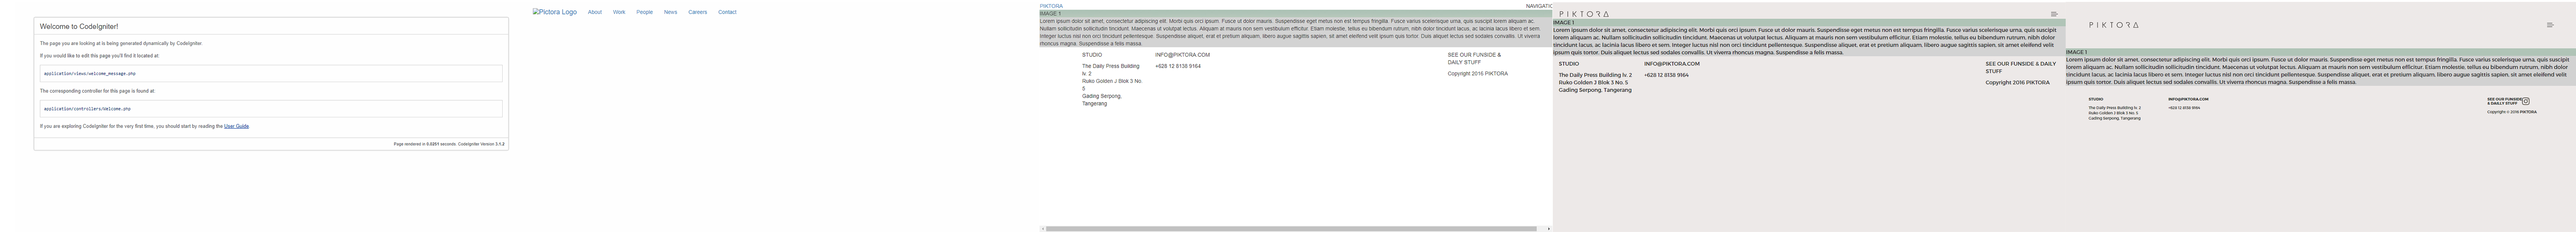
\includegraphics[scale=0.3]{Gambar/Untitled-1.png}
	\caption{\textit{Screenshot} proyek Piktora pada \textit{commit} 315d374 (31 Oktober 2016) - \textit{commit} 5c59916 (8 November 2016).}
	\label{fig:c1}
\end{figure}


\begin{figure}[H]
	
		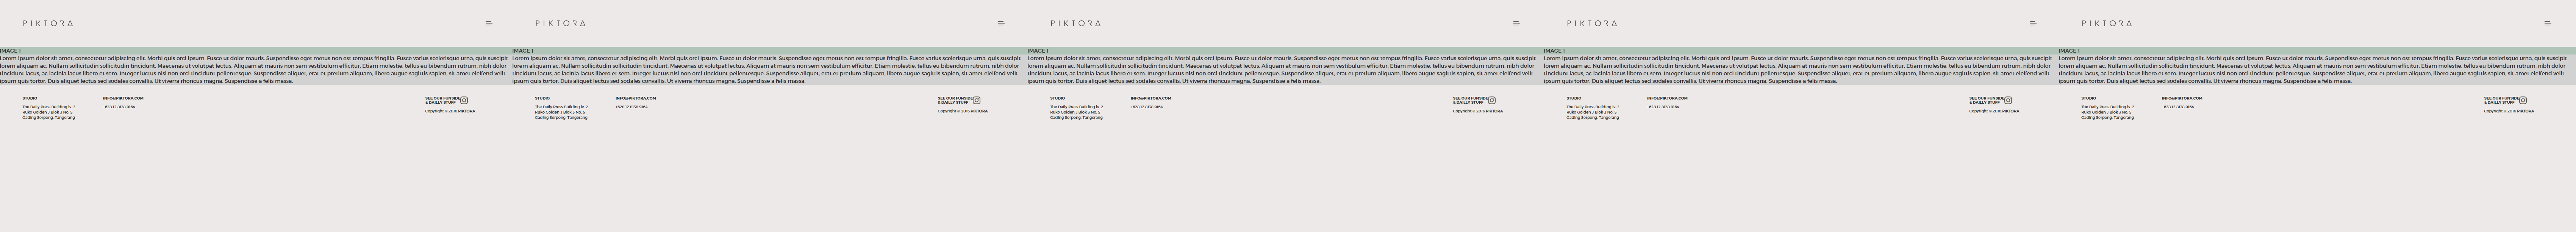
\includegraphics[scale=0.3]{Gambar/Untitled-2.png}
	\caption{\textit{Screenshot} proyek Piktora pada \textit{commit} 7738380 (8 November 2016) - \textit{commit} 3caf535 (15 November 2016).}
	\label{fig:c2}
\end{figure}

\begin{figure}[H]
	
		
\includegraphics[scale=0.3]{Gambar/Untitled-3.png}
	\caption{\textit{Screenshot} proyek Piktora pada \textit{commit} c5eb3b6 (15 November 2016) - \textit{commit} 3eb7af8 (21 November 2016).}
	\label{fig:c3}
\end{figure}

\begin{figure}[H]
	
		
\includegraphics[scale=0.3]{Gambar/Untitled-4.png}
	\caption{\textit{Screenshot} proyek Piktora pada \textit{commit} e87e84b (22 November 2016) - \textit{commit} f0f7270 (23 November 2016).}
	\label{fig:c4}
\end{figure}

\begin{figure}[H]
	
		
\includegraphics[scale=0.3]{Gambar/Untitled-5.png}
	\caption{\textit{Screenshot} proyek Piktora pada \textit{commit} 57a239b (23 November 2016) - \textit{commit} 0fcd958 (28 November 2016).}
	\label{fig:c5}
\end{figure}

\begin{figure}[H]
	
		
\includegraphics[scale=0.3]{Gambar/Untitled-6.png}
	\caption{\textit{Screenshot} proyek Piktora pada \textit{commit} add3974 (28 November 2016) - \textit{commit} 0fe9aaf (29 November 2016).}
	\label{fig:c6}
\end{figure}

\begin{figure}[H]
	
		
\includegraphics[scale=0.3]{Gambar/Untitled-7.png}
	\caption{\textit{Screenshot} proyek Piktora pada \textit{commit} f2326dd (29 November 2016) - \textit{commit} c4e9576 (2 Desember 2016).}
	\label{fig:c7}
\end{figure}

\begin{figure}[H]
	
		
\includegraphics[scale=0.3]{Gambar/Untitled-8.png}
	\caption{\textit{Screenshot} proyek Piktora pada \textit{commit} 02d04f1 (5 Desember 2016) - \textit{commit} eb49c2b (6 Desember 2016).}
	\label{fig:c8}
\end{figure}


\begin{figure}[H]
	
		
\includegraphics[scale=0.3]{Gambar/Untitled-9.png}
	\caption{\textit{Screenshot} proyek Piktora pada \textit{commit} ace1988 (6 Desember 2016) - \textit{commit} c83f4aa (15 Desember 2016).}
	\label{fig:c9}
\end{figure}

\begin{figure}[H]
	
		
\includegraphics[scale=0.3]{Gambar/Untitled-10.png}
	\caption{\textit{Screenshot} proyek Piktora pada \textit{commit} 57f5ea4 (15 Desember 2016) - \textit{commit} 1880a88 (5 Januari 2017).}
	\label{fig:c10}
\end{figure}

\begin{figure}[H]
	
		
\includegraphics[scale=0.3]{Gambar/Untitled-11.png}
	\caption{\textit{Screenshot} proyek Piktora pada \textit{commit} 286aa78 (16 Januari 2017) - \textit{commit} 38711f0 (17 April 2017).}
	\label{fig:c11}
\end{figure}


\begin{figure}[H]
	
		
\includegraphics[scale=0.3]{Gambar/Untitled-12.png}
	\caption{\textit{Screenshot} proyek Piktora pada \textit{commit} 9f041ef (15 Mei 2017) - \textit{commit} 89000be (12 Januari 2018).}
	\label{fig:c12}
\end{figure}





\end{enumerate}
\section{Pengujian}
\label{sec:pengujian}

